\chapter{Benutzerhandbuch} 
\label{chap:Benutzerhandbuch}

\section{Einen Mikrocontroller austauschen}
Für unser Projekt sollen alle notwendigen Programmbestandteile sowie die gesamte
Website auf dem Microcotnroller gespeichert werden. Der beim AVR-Net-IO
mitgelieferte ATmega32 bietet hierfür jedoch nicht ausreichend Speicher.
Wir haben uns deswegen für den aus der gleichen Baureihe stammenden ATmega644P
entschieden der mit seinen 64KB Programmspeicher den doppelten Speicherplatz
bietet als der kleinere ATmeag32.

Für den Wechsel ist es notwendig, den alten Controller vom Sockel zu entfernen
und den neuen Controller einbauen zu können. Hierfür gibt es spezielle
Werkzeuge doch wenn man beim Vorgang Vorsicht walten lässt, kann man den
Controller auch mit einem kleinen möglichst breiten Schlitzschraubendreher
entfernen. Dazu zuerst den Mikrocontroller vorsichtig mit dem Schraubendreher
als Hebel wie in Abbildung \ref{ausbau1} lösen.

\begin{figure}[H]
\centering
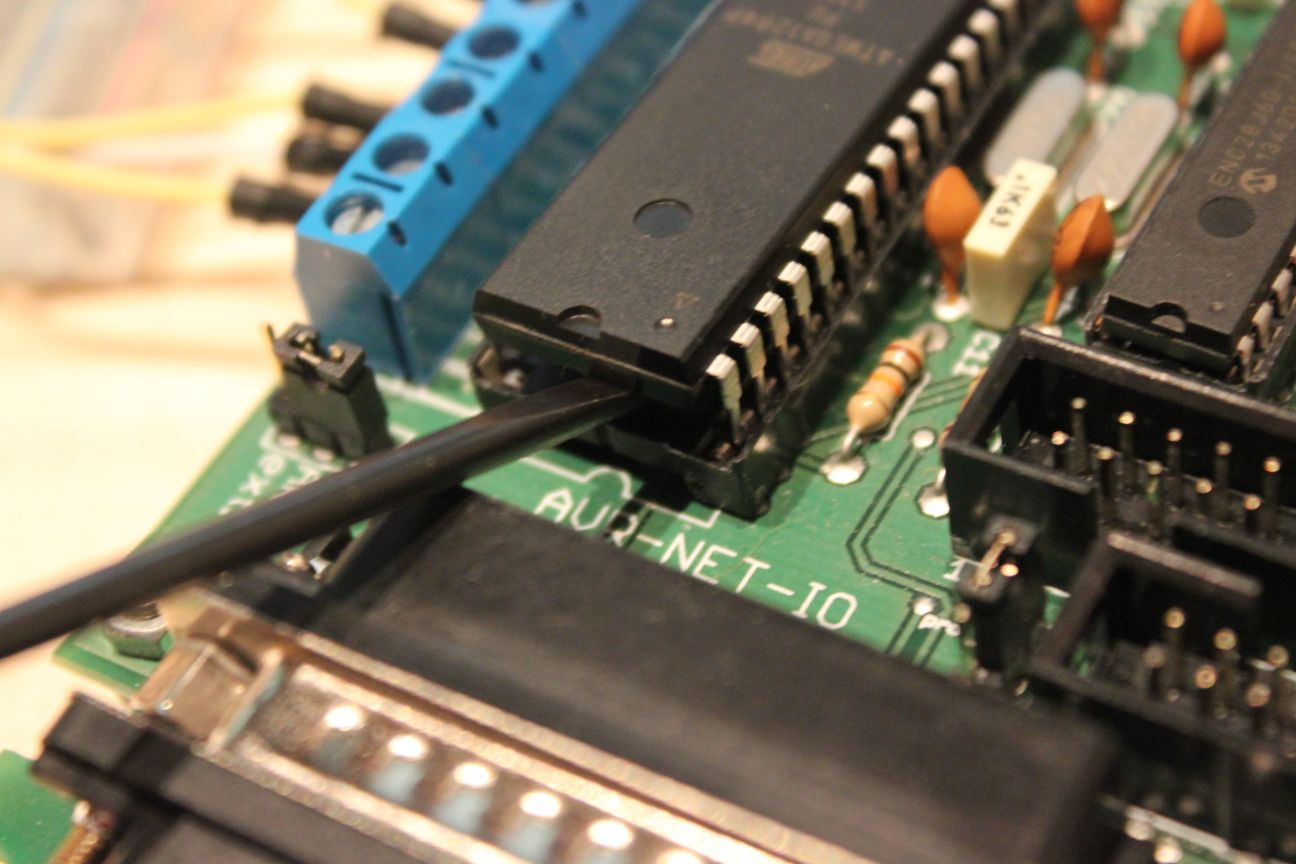
\includegraphics[width=13cm]{content/pictures/Anleitung/tauscheProzessor/1_Hebel.jpg}
\caption{Schraubendreher am Controller}
\label{ausbau1}
\end{figure}

Zum einfachen lösen kann der Hebel auch von der anderen Seite angesetzt
werden. Anschließend den gelösten Prozessor abziehen.

\begin{figure}[H]
\centering
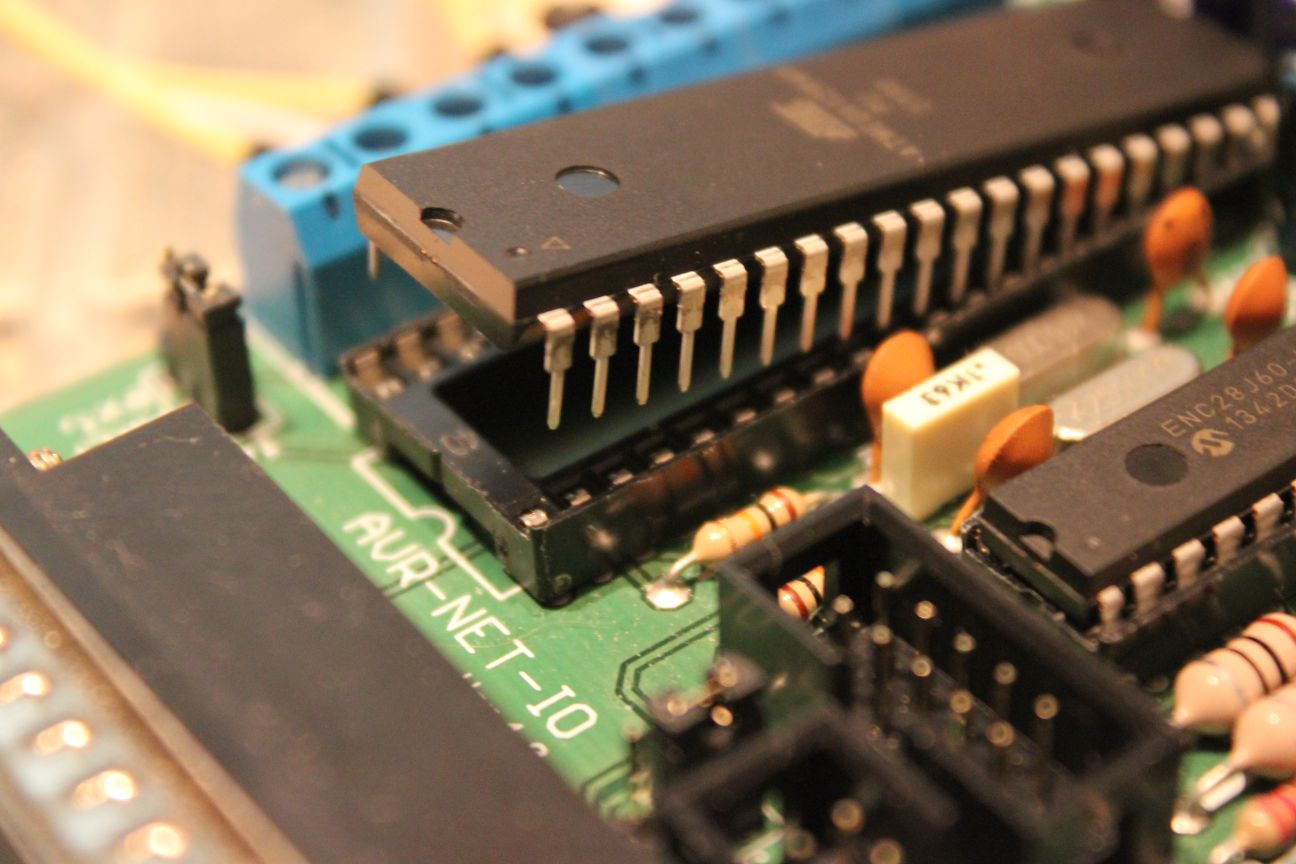
\includegraphics[width=13cm]{content/pictures/Anleitung/tauscheProzessor/2_Geloest.jpg}
\caption{Der gelöste Mikrocontroller}
\label{ausbau2}
\end{figure}

Nachdem der Mikrocontroller entfernt wurde hat man einen guten Blick auf den
Sockel (Abb. \ref{ausbau3}).

\begin{figure}[H]
\centering
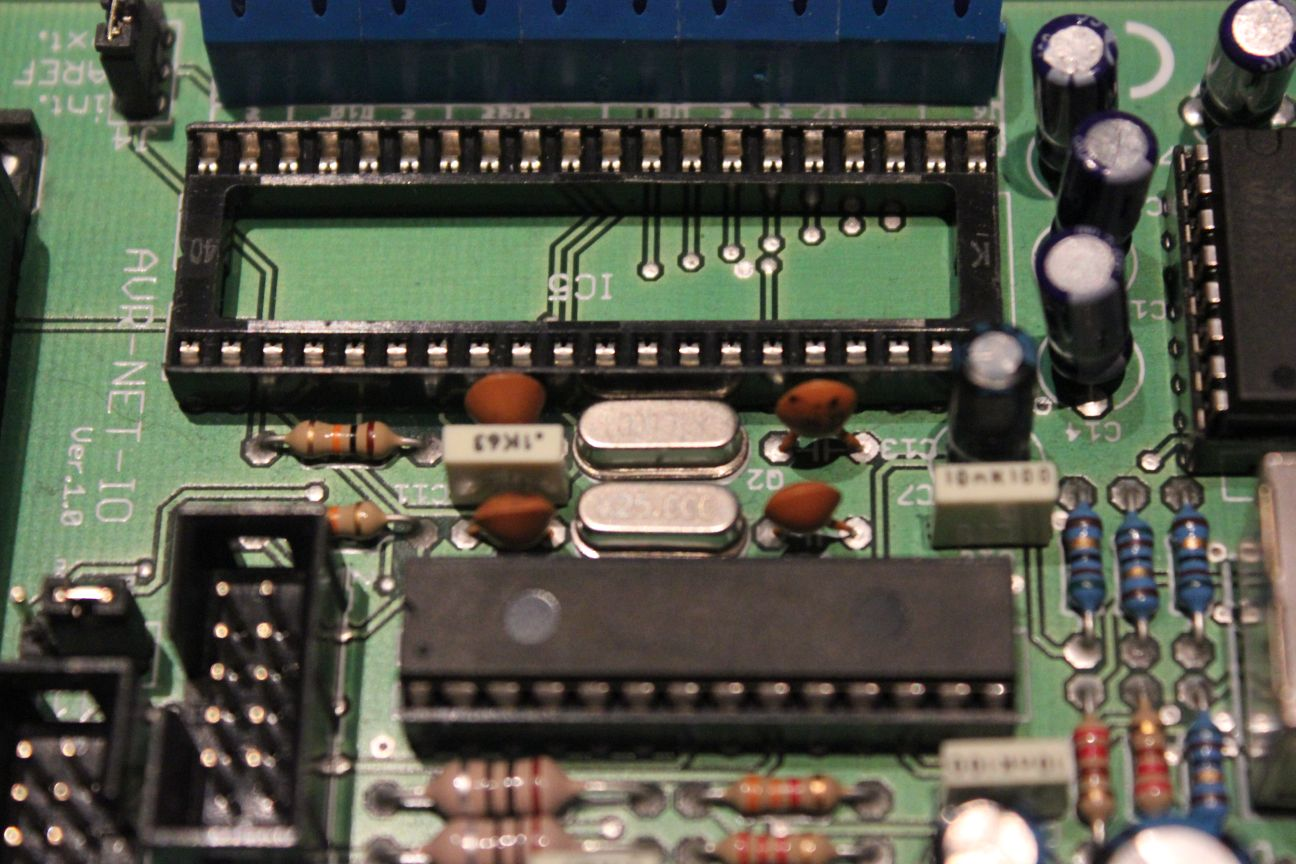
\includegraphics[width=13cm]{content/pictures/Anleitung/tauscheProzessor/3_Sockel.jpg}
\caption{Der Sockel auf dem AVR-Net-IO}
\label{ausbau3}
\end{figure}

Beim Einbau ist unbedingt darauf zu achten den neuen Mikrocontroller entsprechend
der D-Förmige Einkerbung in den Sockel zu setzen. (Siehe Abbildung \ref{ausbau4})

\begin{figure}[H]
\centering
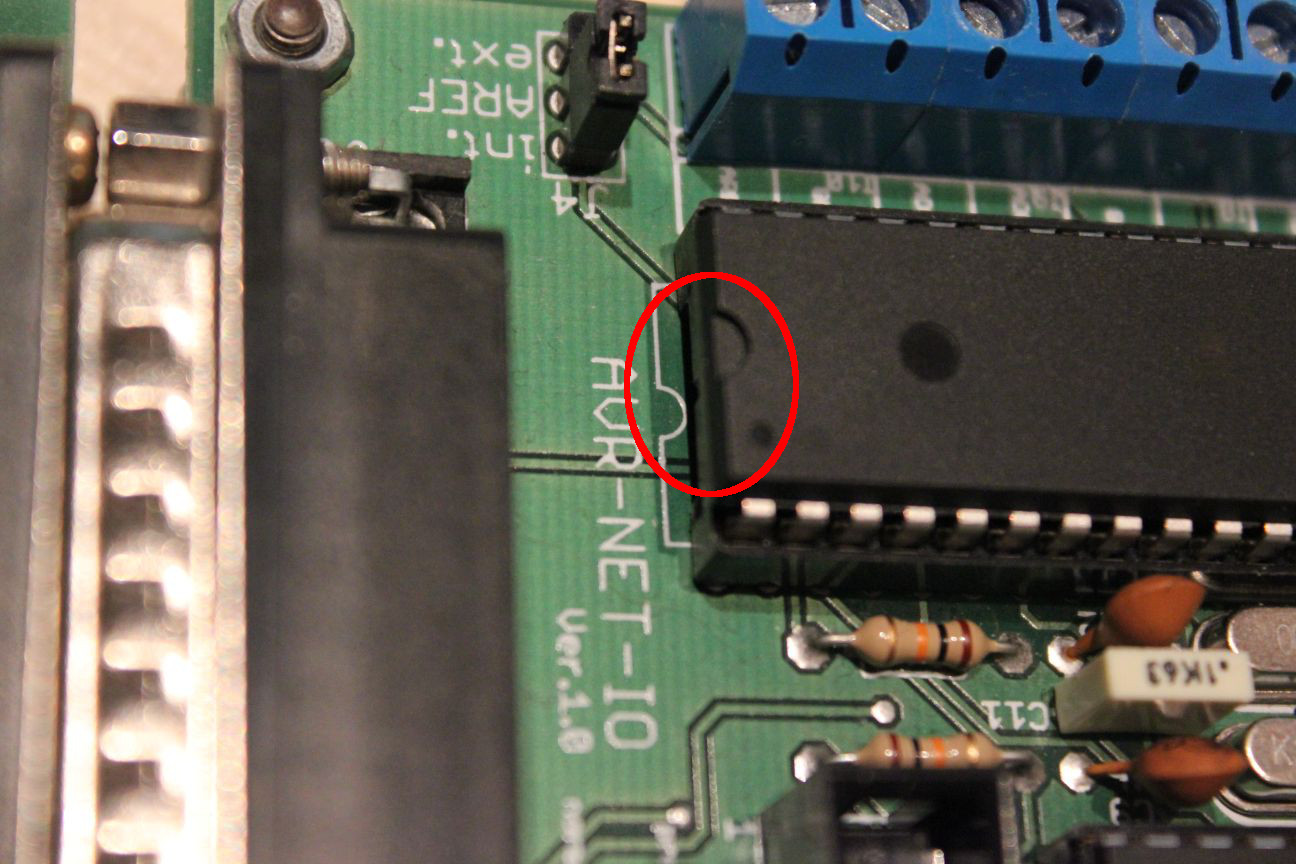
\includegraphics[width=13cm]{content/pictures/Anleitung/tauscheProzessor/4_Markierung.jpg}
\caption{Markierung zum Einbau}
\label{ausbau4}
\end{figure}

\section{ISP-Programmer anschließen}

Der Anschluss des AVRISPmkII Programmers erfolgt über einen 6 Poligen Stecker,
allerdings hat das AVR-Net-IO einen 10 Poligen Stecker. Deswegen wurde hierfür
eigens ein Adapter angefertigt der das ISP Signal von den 6 Polen des Programmers
auf das AVR-Net-IO bring.

\begin{figure}[htp]
\begin{center}
  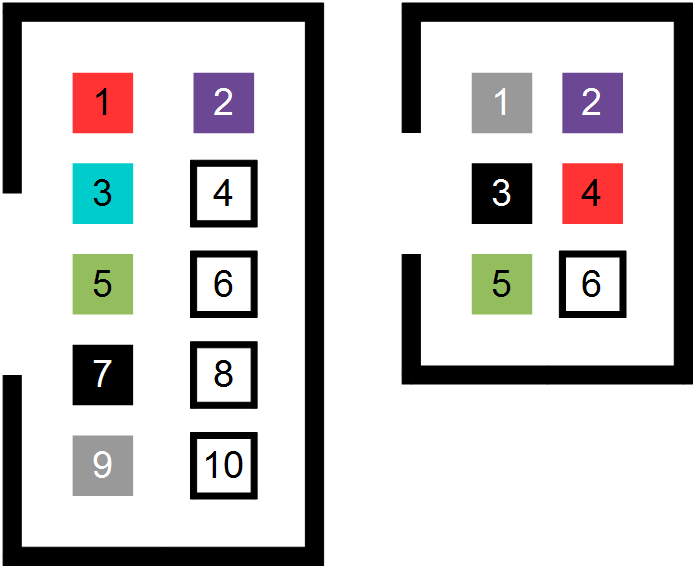
\includegraphics[width=6cm]{content/pictures/Anleitung/ISP-Stecker.png}
  \caption[Schematische Darstellung des ISP Anschlusses]{Schematische Darstellung des ISP Anschlusses (Pin 1 \& 2
  ist auf der Platine markiert)}
  \label{ispanschluss}
\end{center}
\end{figure}

\begin{table}[H]
\centering
\begin{tabular}{|l|l|} \hline
	 \textbf{10-poliger Anschluss} & \textbf{6-poliger Anschluss} \\ \hline
	 1 MOSI & 1 MISO \\ \hline
	 2 VCC & 2 VCC \\ \hline
	 3 - (*) & 3 SCK \\ \hline
	 4,6,8,10 GND & 4 MOSI \\ \hline
	 5 RESET & 5 RESET \\ \hline
	 7 SCK & 6 GND \\ \hline
	 9 MISO &   \\ \hline
\end{tabular}
\caption{Die Pinbelegung für den 6 und 10 poligen Anschluss \cite{mikrocontroller.isp}}
\label{pinbelegung}
\end{table}

\begin{figure}[htp]
\begin{center}
  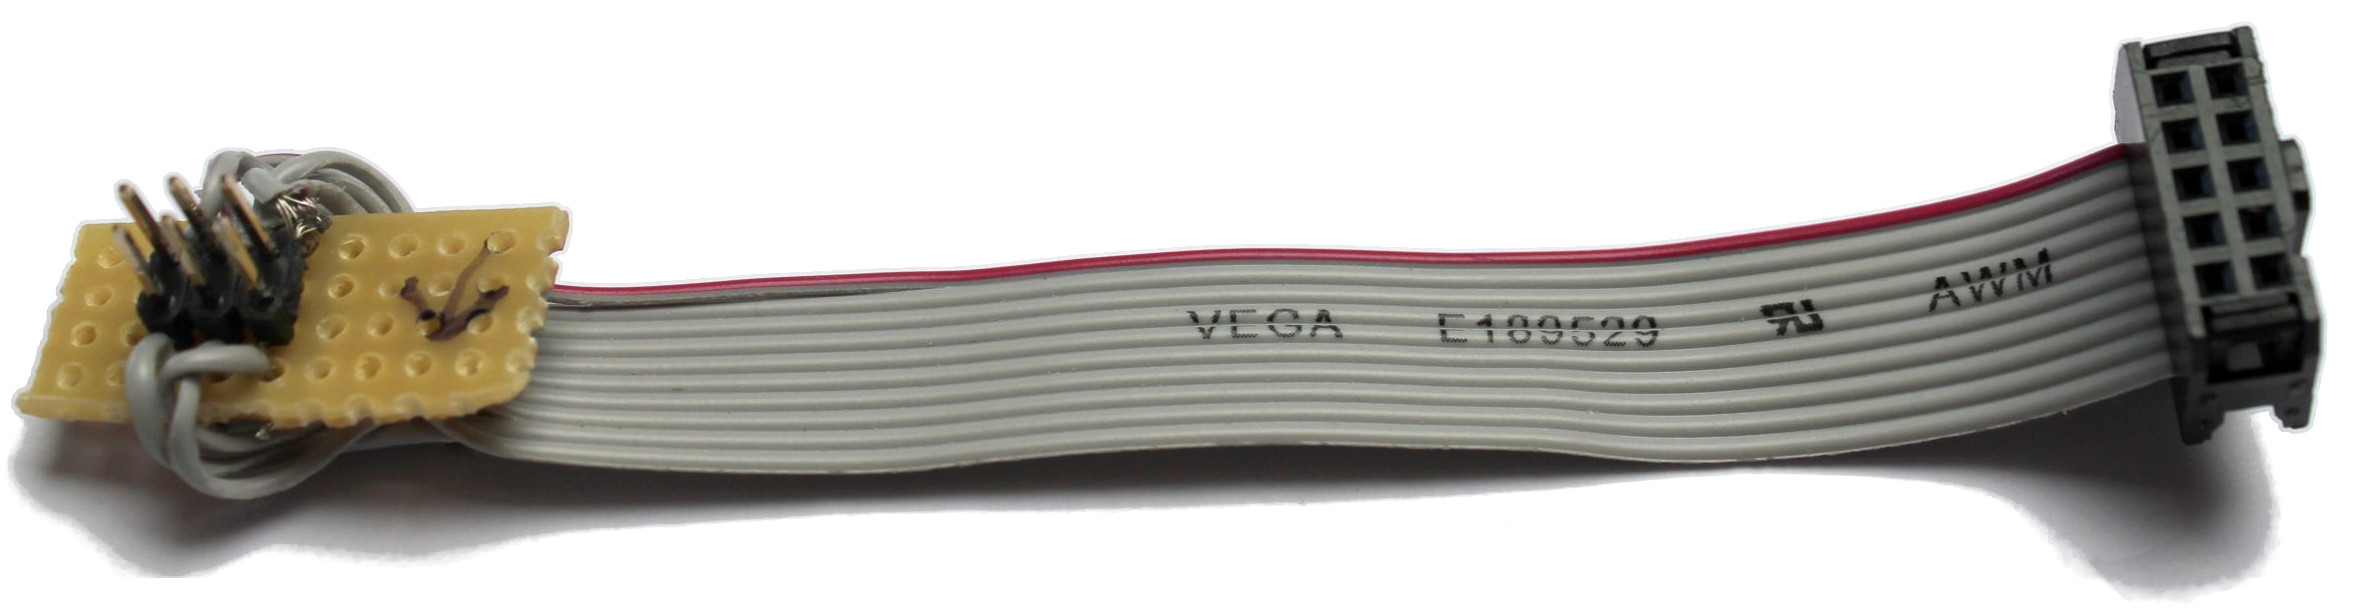
\includegraphics[width=10cm]{content/pictures/Anleitung/adapter.jpg}
  \caption{Der Adapter}
  \label{adapter}
\end{center}
\end{figure}

Mit dem angefertigtem Adapter kann der Debugger anschließend ganz einfach mit
dem Board verbunden werden. Wenn der Mikrocontroller richtig, wie im nächsten Schritt
beschrieben, konfiguriert ist, kann der Programmer auch in Atmel Studio
verwendet werden.

\section{Einrichten eines neuen Mikrocontrollers}
\label{Chapt:Einrichten}

Für einen neuen Chip ist es anfangs notwendig die Fuse-Bits richtig zu setzen,
damit der Chip Ordnungsgemäß Arbeitet.
Dies ist jedoch im AtmelStudio nicht Möglich, da es nicht möglich ist die exakte
Geräte-Signatur auszulesen.
Das Problem liegt darin, das Standartmäßig die Fuses auf den internen
Quarz-Kristall gesetzt sind und nicht auf den Externen Kristall des
AVR-NET-IO Boards.
Beim versuch die Fuse-Bits zu setzen wird man im Atmel Studio mit der
Fehlermeldung aus Abbildung \ref{Einrichten.error} begrüßt.

Abhilfe Schafft hier die Alternative Programmiersoftware AVRDUDE, mit ihr ist
es Möglich die Fuse-Bits zu ändern. Unter Linux kann dieser einfach über die
Paketquellen installiert werden, für ein Windows Betriebssystem kann eine
ausführbare Kommandozeilen-Anwendung auf der Projekt-Website heruntergeladen
werden \url{http://savannah.nongnu.org/projects/avrdude}. Zusätzlich muss für
Windows noch libusb-win32 (\url{http://sourceforge.net/projects/libusb-win32/})
vorhanden sein, das der Programmer mit den gewählten Parametern verwendet werden
kann. Eine ausführliche Anleitung gibt es hier:
\url{http://eliaselectronics.com/using-the-avrispmkii-with-avrdude-on-windows/}

\begin{figure}[H]
\centering
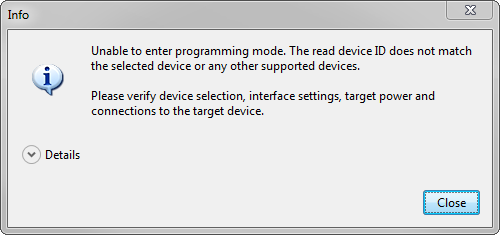
\includegraphics[width=13cm]{content/pictures/Anleitung/neuerProzessor/AnleitungNeuerProzessor2_fehler.png}
\caption{DeviceProgramming}
\label{Einrichten.error}
\end{figure}

Die in Folgendem Beispiel angezeigten Befehle sind die von uns verwendeten Fuse
Einstellungen. Für eine genauere Beschreibung wofür die einzelnen Fuse-Bits
verwendet werden, ist der Abschnitt \ref{chap:Fuse} Fusebits im Kapitel 
Hardware.

Anschließend kann der Mikrocontroller zusammen mit dem AV-Net-IO und AtmelStudio
Programmiert werden. Der Verwendete Mikrocontroller wird jetzt richtig erkannt,
da es auch keine Probleme mit der Gerätesignatur gibt.

\begin{table}[H]
\begin{tabular}{| p{.24\textwidth} | p{.76\textwidth} |}
\hline
Auslesen Linux:& sudo avrdude -P usb -p m644p -c avrispmkII  -U lfuse:r:-:h -U hfuse:r:-:h -B 22 \\ \hline
Setzen Linux:& sudo avrdude -P usb -p m644p -c avrispmkII -U lfuse:w:0xFF:m -U hfuse:w:0xD6:m -B 22 \\ \hline
Auslesen Windows:& avrdude.exe -p m644p -c avrispmkII -U lfuse:r:-:h -U hfuse:r:-:h -B 22 \\ \hline 
Setzen Windows:& avrdude.exe -p m644p -c avrispmkII -U lfuse:w:0xFF:m -U hfuse:w:0xD6:m -B 22 \\ \hline
\end{tabular}
\caption{Auslesen und setzen von Fuse-Bits des ATmega644P mit AVRDUDE}
\label{ParameterAvrdude1}
\end{table}

\begin{figure}
\centering
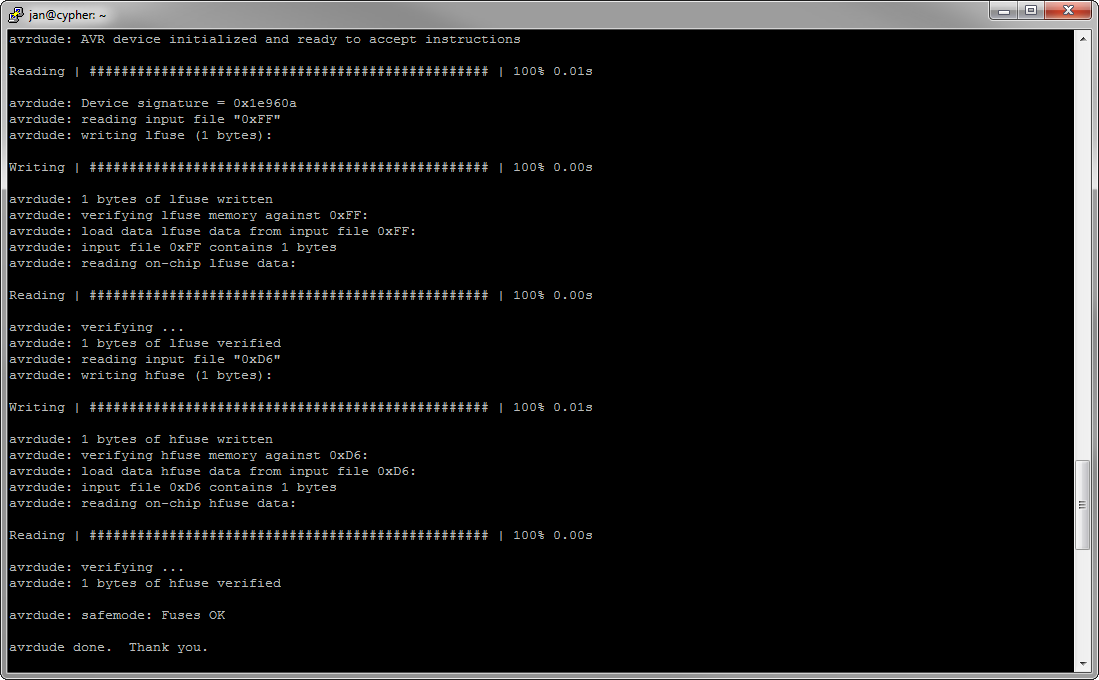
\includegraphics[width=13cm]{content/pictures/Anleitung/neuerProzessor/avrOutput.png}
\caption{AVRDUDE Ausgabe}
\end{figure}

\begin{table}
\begin{tabular}{| p{.35\textwidth} | p{.65\textwidth} |}
\hline
-p partno & This is the only option that is mandatory for every invocation of
avrdude.  It specifies the type of the MCU connected to the programmer. These
are read from the config file.  If avrdude does not know about a part that you
have, simply add it to the config file (be sure and submit a patch back to the
author so that it can be incorporated for the next version). \newline
\textbf{m32 $\Rightarrow$ ATmega32} \newline 
\textbf{m644p $\Rightarrow$ ATmega644P} \newline
\textbf{m1284p $\Rightarrow$ ATmega1284P} \\ \hline
-P port & Use port to identify the device to which the programmer is attached. \textbf{usb für den AVRISP MKII}  \\ \hline 
-c programmer-id & \textbf{avrispmkII für den AVRISP MKII} \\ \hline
-U \hbox{memtype:op:filename:filefmt} &  
The \textrm{memtype} field specifies the memory type to operate on.\newline
\textbf{hfuse} The high fuse byte.\newline
\textbf{lfuse} The low fuse byte.\newline
The \textrm{op} field specifies what operation to perform:\newline
\textbf{r} read device memory and write to the specified file\newline
\textbf{w} read data from the specified file and write to the device memory \newline
The filename field indicates the name of the file to read or write.  The format field is optional and contains the format of the file to read or write. \newline
\textbf{Hier die Bytes die gesetzt werden 0xFF bzw 0xD6} \\ \hline
-B bitclock & Specify the bit clock period for the JTAG interface or the ISP clock \\ \hline
\end{tabular}
\caption{Auszug AVRDUDE Parameter}
\label{parameterAvrdude2}
\end{table}
\newpage

\section{HTML Header Compiler}
\label{chap:benutzerhandbuch.HHC}

Da der HTML Header Compiler in Java entwickelt wurde muss für die Verwendung die
Java Laufzeitumgebung ab Version 6 installiert sein. Zum Ausführen des Compiler
muss zuerst mit einer Konsole in den Entsprechenden Ordner navigiert werden.
Anschließend kann mit folgendem Befehl die Datei ausgegeben werden. 
\\

\framebox[1.1\width]{java -jar hhc.jar -in <INPUT FOLDER> -out <OUTPUT FILE>} 
\\

Die Angaben in den spitzen Klammern müssen durch den entsprechenden Pfad und
die entsprechende Datei ausgetauscht werden. Standardmäßig optimiert der
HTML Header Compiler die eingegebenen Dateien, falls dies nicht gewünscht ist
gibt es zusätzlich zu den vorgegebenen Optionen weitere Flags
die gesetzt werden können. Hier alle Parameter im Überblick:

\begin{table}[H]
\begin{tabular}{| p{.24\textwidth} | p{.76\textwidth} |}
\hline
-in, -input & Der Eigabepfad mit allen für die Website benötigten Dateien. z.B. \textrm{-in "Webseite"} \\ \hline 
-out, -output & Die Ausgabe Headerdatei z.B. \textrm{-out "Webserver/webpage.h"} \\ \hline
-v, -verbose &  Gibt die ausgegebenen Dateien auf der Console aus. \\  
 \hline 
 -n, -newline & Behält die Formatierung für den Zeilenvorschub, Tabulator
 oder Wagenrücklauf in den HTML und JS Dateien (\textbackslash n and
 \textbackslash r \textbackslash t).
 Benötigt dadurch abhängig von der Website mehr Speicher, ermöglicht aber ein
 einfacheres Debuggen von eingebundenem JavaScript Code.  \\ \hline
\end{tabular}
\caption{Parameter des HTML Header Compiler}
\label{parameterHHC}
\end{table}

Um die Entwicklung zu vereinfachen ist es hilfreich, wenn für den Parameteraufruf
des HTML Header Compilers ein einfaches Schell- oder Batch-Script erstellt, das
die Dateien aus dem Ordner für die Website als Headerdatei in den Ordner für den
Webserver schreibt. Falls eine Änderung an der Website vorgenommen wurde muss
vor dem Programmieren des Mikrocontrollers lediglich der \ac{HHC} Ausgeführt
werden.

\begin{figure}[H]
\lstinputlisting[language=sh]{content/code/buildwebpage.sh}
\caption{BuildWebpage.sh für Linux}
\label{output}
\end{figure}

\begin{figure}[H]
\lstinputlisting[language=sh]{content/code/buildwebpage.bat}
\caption{BuildWebpage.bat für Windows}
\label{output}
\end{figure}

\section{Konfiguration des Webservers}

Die Einstellung des Webservers erfolgt über die \textrm{config.h} Datei. In der
\textrm{config.h} Datei, können Zum einen die verschiedenen Pins der Ports als Ein oder
Ausgang definiert werden. Dabei gibt es ein paar Eigenheiten zu beachten:
\begin{itemize}
  \item OUTA steht für den A Port, hier ist du beachten, das dieser Port die
  Analog zu Digital Wandler beherbergt. Mit aktiviertem Wandler ist es nicht
  möglich die Pins des Ports funktionierend als Ausgänge zu schalten, da die
  Spannung nicht gehalten wird.
  \item OUTB ist nur mit Vorsicht zu genießen. Hier handelt es sich um den Port
  der auf dem AVR-Net-IO für die Neztwerkkomunikation genutzt wird. Deswegen
  wird Port B auch nicht Standardmäßig definiert.
  \item OUTC dieser Port wird von Polin standardmäßig für die Ausgänge verwendet
  und ist von uns bereits so Modifiziert. Der gesamte Port wird auf dem
  AVR-NET-IO über den 25Pin D-Sub Stecker geleitet. Wenn der Fuse-Bit für JTag
  geschaltet ist werden 4 Pins des C Ports für das JTag Interface verwendet.
  \item OUTC Der C Port liegt auf dem AVR-Net-IO auf dem EXT Anschluss und ist
  für erweiterte Peripherie geplant, so kann hier ein Cardreader oder ein
  Erweiterungsboard angeschlossen werden.
\end{itemize}
Weiter kann die gewünschte IP-Adresse eingestellt werden, unter der das Gerät
erreicht werden kann. Wichtig ist hier, das kein anderes Gerät die selbe Adresse
im Netzwerk verwendet. Auch kann die Router IP-Adresse und Netzmaske angegeben
werden. Eine weitere Wichtige Einstellung ist die verwendete Mac Adresse
des Netzwerk Controllers. Diese wird über die Variablen MYMAC1-6 Definiert.

\section{Debuggen über JTAG}

Der JTAGICEmkII Debugger von Atmel, den wir für unser Projekt gestellt bekommen
haben, unterstützt neben ISP auch JTAG. Allerdings werden für den Anschluss von
JTAG andere Pins benötigt als für den Anschluss eines ISP Programmers.

\begin{table}
\begin{longtable}{|l|l|l|p{8.8cm}|}\hline 
Pin & Signal & I/O & Description \\ \hline 
1 & TCK & Output & Test Clock, clock signal from JTAGICE mkII to target JTAG port \\ \hline 
2 & GND & - & Ground \\ \hline 
3 & TDO & Input & Test Data Output, data signal from target JTAG port to JTAGICE mkII \\ \hline 
4 & Vtref & Input & Target reference voltage. Also used to power level converter inputs. \\ \hline 
5 & TMS & Output & Test Mode Select, mode select signal from JTAGICE mkII to target JTAG port \\ \hline 
6 & nSRST & Out/-In-put & Open collector output from adapter to the target system reset. This pin is also an input to the adapter so that the reset initiated on the target application board may be reported to the JTAGICE mkII \\ \hline 
7 & - & - & Not connected \\ \hline 
8 & nTRST & NC(Output) & Not connected, reserved for compatibility with other equipment (JTAG port reset) \\ \hline 
9 & TDI & Output & Test Data Input, data signal from JTAGICE mkII to target JTAG port \\ \hline 
10 & GND & - & Ground \\ \hline 
\end{longtable}
\caption{JTAG Connections \cite{JTAGICEmkII.Quick}}
\label{jtag.Connections}
\end{table}

\begin{figure}[htp]
\begin{center}
  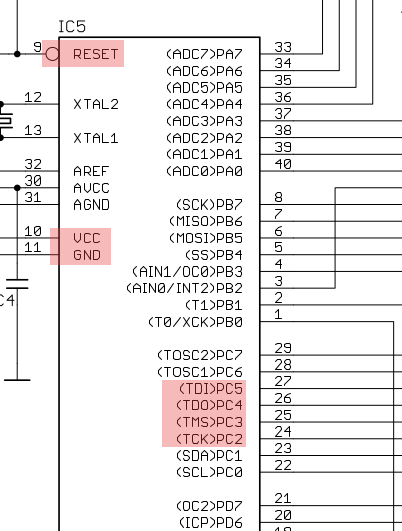
\includegraphics[width=6cm]{content/pictures/jatgPins.png}
  \caption{JTAG Pins}
  \label{jtag.pins}
\end{center}
\end{figure}

Die in Tabelle \ref{jtag.Connections} gezeigten Pins entsprechen der Belegung
der 10 Anschlüssen des JTAGICEmkII. Diese müssen mit den Pins 2-5 des C Ports, dem
Reset Pin, Ground und VCC verbunden werden (Abbildung \ref{jtag.pins}). Die Pins 7 \& 8
des JTAGICEmkII werden nicht mit dem Mikrocontroller verbunden.\\
\\
Damit \ac{JTAG} funktioniert muss der Entsprechende JTAG Fuse-Bit gesetzt sein.
Dabei ist zu beachten das die Pins 2-5 am Port C des Mikrocontroller nicht für
Ein- oder Ausgaben verwendet werden können sondern bei aktivierten Fuse-Bit
gesperrt sind. Als weiterer Hinweis ist zu beachten, dass die Verwendete
Schnittstelle in den Projekt Einstellungen umgestellt werden muss. Nach
Korrekter Verbindung, die im Device Manager überprüft werden kann kann das
Programm auf dem Mikrocontroller debuggt werden.

\section{WinAVR Projekt zu Atmel Studio}

%TODO Beispielexport

\section{Die Website}

Die Webseite ist in 3 Tabs eingeteilt. 

\subsection{Der Status Tab}
In dem Status Tab ist die Übersicht der
einzelnen Pins und Ports des Boarders. Beim darüberhinwegfahren mit der
Maus erscheint auf der rechten Seite des Browser eine Sidebar mit den
detailierten Inforamtionen zu diesem Pins. Nicht alle Pins oder Ports sind
klickbar, da diese vom System deaktiviert sind. Hier können die Pins oder Ports
als Favoriten gespeichert werden. Genauso können Werte und Skripte der einzelnen
Pins oder Ports geändert werden.

\subsection{Der Favoriten Tab}
Hier werden tabellarisch die ausgewählten Pins oder Ports angezeigt, auch hier
können wieder pinspezifische Modifikationen vorgenommen werden. Löschen der
Favoriten setzt den Pin auf die Standardeinstellungen zurück und ist nicht mehr
in Favoritenliste vorhanden. Pins können wieder über den Status Tab hinzugefügrt
werden.

\subsection{Der Einstellungs Tab}
Im Einstellungs Tab werden die Einstellungen vorgenommen. Hier sind auch die
Informationen über das Board, Version der Webseite und Autoren abrufbar. Die
Import/Export Funktion ermöglicht die Datenbank, in der die benutzereinstelungen
und Favoriten untergebracht sind zu expotieren und auf einem anderen System zu
importieren. Die Aktualisierungsrate bestimmt wie schnell sich die Seite
aktualisert, das ist die einzige Einstellungen die vorgenommen werden kann.

\subsection{Bespiele: Skripte}
Einige Beispielskripte, die nur noch für die passenden Pins und Ports angepasst
werden müssen. Diese Skripte können kopiert und das dafür vorgesehene Fenster
im Webbrowser eingefügt werden.

\subsubscetion*{ein Licht blinken}
Lässt den Pin C0 blinken:\newline
\begin{lstlisting}
if (getValue('C0') == "0") {
	setValue('C0',1);
} else {
	setValue('C0',0);
}
\end{lstlisting}

\subsubscetion*{mehrer Lichter blinken}
dieses Skript lässt die Lichter an Pin D2-D7 blinken:\newline
\begin{lstlisting}
if (getValue('D2') == "1") {
	setValue('D2',0);
	setValue('D3',1);
	setValue('D4',0);
	setValue('D5',1);
	setValue('D6',0);
	setValue('D7',1);
} else {
	setValue('D2',1);
	setValue('D3',0);
	setValue('D4',1);
	setValue('D5',0);
	setValue('D6',1);
	setValue('D7',0);
}
\end{lstlisting}

\subsubscetion*{Umwandeln in digitale Werte}
dieses Skript wandelt den Input des Sensors A5 in digitale Werte um:\newline
\begin{lstlisting}
setValue('D2',0);
setValue('D3',0);
setValue('D4',0);
setValue('D5',0);
setValue('D6',0);
setValue('D7',0);


var value = getValue('A5');

if (value > 869) {
	setValue('D2', 1);
}
if (value > 719) {
	setValue('D3', 1);
}
if (value > 569) {
	setValue('D4', 1);
}
if (value > 419) {
	setValue('D5', 1);
}
if (value > 269) {
	setValue('D6', 1);
}
if (value > 119) {
	setValue('D7', 1);
}
\end{lstlisting}

\subsubscetion*{Lauflicht}
dieses Skript bildet ein Lauf von Lichter die nach einander an und wieder
ausgeschaltet werden:\newline
\begin{lstlisting}
var count = getDb("count", "0");

switch (count) {
case "0":
	setValue('D7',0);
	setValue('D2',1);
	console.log(count);
	count = 1;
	break;
case "1":
	setValue('D2',0);
	setValue('D3',1);
	count = 2;
	break;
case "2":
	setValue('D3',0);
	setValue('D4',1);
	count = 3;
	break;
case "3":
	setValue('D4',0);
	setValue('D5',1);
	count = 4;
	break;
case "4":
	setValue('D5',0);
	setValue('D6',1);
	count = 5;
	break;
case "5":
	setValue('D6',0);
	setValue('D7',1);
	count = 0;
	break;
} 

putDb("count", count);
\end{lstlisting}

\subsubscetion*{Automatischer Countdown}
Diese Skript lässt die 7 Segment Anzeige nacheinander durchiterieren.
Daraus entsteht ein Countdown:\newline
\begin{lstlisting}
var count = getDb("count", "0");

var set7Digit = function(number){
	var pins = [[0,0,1,0,0,0,0],
				[0,1,1,1,1,1,0],
				[0,0,0,1,0,0,1],
				[0,0,0,1,1,0,0],
				[0,1,0,0,1,1,0],
				[1,0,0,0,1,0,0],
				[1,0,0,0,0,0,0],
				[0,0,1,1,1,1,0],
				[0,0,0,0,0,0,0],
				[0,0,0,0,1,0,0]]

	setValue('C0',pins[number][0]);
	setValue('C1',pins[number][1]);
	setValue('C2',pins[number][2]);
	setValue('C3',pins[number][3]);
	setValue('C4',pins[number][4]);
	setValue('C5',pins[number][5]);
	setValue('C6',pins[number][6]);
};

switch (count) {
case "0":
	set7Digit(count);
	count = 1;
	break;
case "1":
	set7Digit(count);
	count = 2;
	break;
case "2":
	set7Digit(count);
	count = 3;
	break;
case "3":
	set7Digit(count);
	count = 4;
	break;
case "4":
	set7Digit(count);
	count = 5;
	break;
case "5":
	set7Digit(count);
	count = 6;
	break;
case "6":
	set7Digit(count);
	count = 7;
	break;
case "7":
	set7Digit(count);
	count = 8;
	break;
case "8":
	set7Digit(count);
	count = 9;
	break;
case "9":
	set7Digit(count);
	count = 0;
	break;
} 

putDb("count", count);
\end{lstlisting}